\documentclass[a4paper]{article} % A4 paper and 11pt font size

\usepackage{braket}
\usepackage{amsmath}
\usepackage{amssymb}
\usepackage{bm}
\usepackage[utf8]{inputenc}
\usepackage{verbatim}
\usepackage{tikz}
\usepackage{pgfplots}
\usepackage{siunitx}
\usepackage{pgfornament}
\usepackage{hyperref}
\usepackage{fancyhdr}
\usepackage{pdflscape}
\usepackage{bm}
\usepackage{enumitem}
\usepackage[a4paper]{geometry}
\usepackage{framed}
\usepackage{gensymb}


%for side-by-side figures
\usepackage{graphicx}
\usepackage{caption}
\usepackage{subcaption}


\setlength{\parindent}{2em}
\setlength{\parskip}{1em}
\renewcommand{\baselinestretch}{1.2}
\newcommand{\ms}[1]{\SI{#1}{M_{\odot}}}

% include this to remove the "References" heading in bibliography
\usepackage{etoolbox}
\patchcmd{\thebibliography}{\section*{\refname}}{}{}{}


\newcommand{\picturesize}[2]
{
\begin{figure}[h]
\centering
\includegraphics[width=#2\textwidth]{#1}
\end{figure}
}


\newgeometry{bottom=4cm}

\begin{comment}
 \geometry{
 a4paper,
 total={210mm,297mm},
 left=40mm,
 right=40mm,
 top=20mm,
 bottom=20mm,
 }
 \end{comment}

%----------------------------------------------------------------------------------------
%	TITLE SECTION
%----------------------------------------------------------------------------------------
\setlength\parindent{0pt} % Removes all indentation from paragraphs - comment this line for an assignment with lots of text


\pagenumbering{arabic}
\begin{document}
\pagestyle{empty}

\newcommand{\HRule}{\rule{\linewidth}{0.5mm}}

\begin{titlepage}

    \begin{center}
        \textsc{}\\[3cm]

        %\HRule \\[0.5cm]
        \pgfornament[width = 0.9\textwidth, symmetry=v]{88}\\[0.75cm]        
        \Huge \textbf{PHYC30019 Astrophysics}\\[0.5cm]
        \huge \textbf{Project 1:} The Birth of Stars\\[0.5cm] 
        \pgfornament[width = 0.9\linewidth]{88}\\[1.5cm]
        %\HRule \\[1.5cm]

        \begin{minipage}{0.5\textwidth}
        \begin{center}

		\vspace{3cm}
        \large By \\[0.75cm]
        \begin{tabular}{rl}
        \Large Braden &\Large \textsc{Moore} \\[0.1cm]
        \Large Jude & \Large \textsc{Prezens} \\    
		\end{tabular}  
		\\[1cm]
        \normalsize \normalfont 
        The University of Melbourne \\[2cm]

        \end{center}
        \end{minipage}

        \vfill

        \large \today
    \end{center}

\newpage
\end{titlepage}
%----------------------------------------------------------------------------------------
\begin{comment}
\pagestyle{fancy}
\pagenumbering{gobble}
\tableofcontents
\newpage
\end{comment}
\pagenumbering{arabic}
\rfoot{\textsc{PHYC30012 Astrophysics}}

\pagestyle{fancy}
\setcounter{page}{1}
\section{Order-of-magnitude estimates}
\subsection{Order-of-magnitude estimate 1}
\begin{framed}
Are there more grains of sand on the beaches of Earth or more stars in the Milky Way?
\end{framed}

\subsubsection{Grains of sand}
We begin by estimating the number of beaches on Earth.
\begin{align*}
\text{no. of continents}&=7\sim 10\\
\text{no. of beaches/continent}&\sim 10,000\\
&\Rightarrow 100,000 \text{ beaches on Earth}
\intertext{We then make an estimate of the average volume of a beach covered by sand\footnotemark}
\text{average length of beach}&=\SI{1000}{m}\\
\text{average width of beach}&=\SI{10}{m}\\
\text{average depth of beach}&=\SI{2}{m}\\
\Rightarrow&=\SI{20,000}{m^3}\text{ of sand per beach}
\intertext{Next we estimate the number of grains of sand in a $\SI{1}{cm^3}$ box to be $\sim 1000$.}
\Rightarrow &1000\text{ grains of sand/} \si{cm^3}\\
\Rightarrow &10^3\times 10^6 \text{ grains of sand/}\si{m^3}
\intertext{We can now estimate the number of grains of sand on the beaches of Earth as}
\text{number of grains of sand}&\sim 100,000\text{ beaches} \times \SI{20,000}{m^3}/\text{beach}\times 10^9\text{ grains/}\si{m^3}\\
&\sim 2\times 10^5 \times 10^5 \times 10^9 \text{ grains}\\
&\sim 2\times 10^{19}\text{ grains}
\end{align*}

 \footnotetext{Width is taken as the distance from the average water level to the grassland/non-sandy area beyond the beach. Depth is taken as the vertical distance from surface sand to the first point below the beach surface where there is no longer sand.}

\subsubsection{Stars}
We begin by determining a rough measure of volume for the Milky Way.
\begin{align*}
\text{diameter of Milky Way}&\sim \SI{100000}{ly}\\
\text{thickness of Milky Way}&\sim \SI{2000}{ly}\\
\Rightarrow \text{volume}&=\pi\left(\frac{\SI{100000}{ly}}{2}\right)^2 \times \SI{2,000}{ly}\\
&\sim \frac{6}{4}\times 10^3\left(10^5\right)^2 \si{(ly)^3}\\
&\sim 1.5\times \SI{d13}{(ly)^3} 
\intertext{We then estimate the average distance between stars. To do this, we take the distance from the Sun to its nearest neighbour as $\sim\SI{4}{ly}$. Using this distance we then suppose that each star exists within a ``starbox'' of dimensions $2\times 2\times \SI{2}{(ly)^3}$.}
\text{Volume per star}&\sim \SI{8}{(ly)^3}/\text{star}\\
\intertext{Now we can estimate the number of stars as:}
\text{Number of stars in the Milky Way}&= \frac{\text{volume of Milky Way}}{\text{volume/star}}\\
&\sim \frac{1.5\times 10^{13}}{8}\\
&\sim\frac{10^{13}}{10}\\
&= \SI{d12}{stars}
\end{align*}

\subsubsection{Conclusion}
From the above, we claim that
\begin{align*}
\text{Number of grains of sand on the beaches of Earth}&\sim 10^{19}\\
\text{Number of stars in the Milky Way}&\sim 10^{12}
\end{align*}

From the rough order-of-magnitude calculations performed, we deduce \emph{there are more grains of sand on the beachs of Earth than there are stars in the Milky Way}. Even though we have made many assumptions as well as liberal rounding of numbers, it is unlikely that these values are more than an order of magnitude greater or smaller than quoted. 

It is validating to note that the common answer for number of stars in the Milky Way is quoted as $\sim 10^{11}$ \cite{StarsInMilkyWay}.

\pagebreak

\subsection{Order-of-magnitude estimate 2}
\begin{framed}
A globular cluster comprises many tens to hundreds of thousands of stars. As they orbit in the galaxy, they are sometimes torn apart by the galaxy's tidal forces. Assuming the same orbits, which will survive longer: a $\SI{d5}{M_\odot}$ cluster of radius $\SI{10}{pc}$, or one with a radius of $\SI{1}{pc}$? What would happen if the second one had a mass instead of $\SI{d4}{M_\odot}$?
\end{framed}

\subsubsection{Tidal force equation}
We consider the tidal force as the difference in gravitational force from the centre of an object to the external point closest to the object causing gravitational attraction. Where $R$ is the distance from the center-of-mass of the gravitational object to the center-of-mass of the object experiencing tidal force, and $\Delta r$ is the distance from that object's center-of-mass to the aforementioned external point, we have

\begin{equation}
F_{\text{tidal}}=F_{\text{grav}}(R)-F_{\text{grav}}(R-\Delta r)
\end{equation}

We know gravitational force is given as
\begin{equation}
F_{\text{grav}}=\frac{GMm}{r^2}
\end{equation}
so we find the expression for tidal force as:
\begin{align}
F_{\text{tidal}}&=\frac{GMm}{R^2}-\frac{GMm}{(R-\Delta r)^2}\nonumber\\
&=GMm\left[\frac{(R-\Delta r)^2-R^2}{R^2 (R-\Delta r)^2}\right]\nonumber\\
&=GMm\left[\frac{\Delta r^2-2R\Delta r}{R^4-2R^3\Delta r +R^2\Delta r^2}\right]\nonumber
\intertext{Assuming $\Delta r \ll R$, and assuming $R$ is large,}
F_{\text{tidal}}&\sim -GMm\left[\frac{2R\Delta r}{R^4}\right]\\
\Rightarrow F_{\text{tidal}}&\sim -\frac{2GMm\Delta r}{R^3}\label{F tidal}
\end{align}

We can also express (\ref{F tidal}) explicitly in only terms of $\Delta r$ and $m$ multiplied by a constant:
\begin{equation*}
F_{\text{tidal}}\propto m\Delta r\label{F tidal prop}
\end{equation*}

\subsubsection{Conclusion}
Clearly, a $\SI{d5}{M_\odot}$ cluster of radius $\SI{1}{pc}$ will experience less tidal force than a cluster of radius $\SI{10}{pc}$ and hence will survive longer. This would also be true if the former had a mass of $\SI{d4}{M_\odot}$; it would then experience 100 times less force than the larger, heavier cluster.


\pagebreak

\subsection{Order-of-magnitude estimate 3}
\begin{framed}
Roughly how far must you look in a particular direction before your line-of-sight intersects with a galaxy?
\end{framed}

We will estimate this by considering the mean free path of a photon. This is given by
\begin{equation}
L=\frac{1}{n\sigma}
\end{equation}
where
\begin{align*}
n&=\text{number density of galaxies in the universe}\\
\sigma&=\text{cross section of galaxy}
\end{align*}

We estimate the number density of galaxies in the universe by using our nearest neighbour as a yardstick:
\begin{align}
n&=\frac{1}{(\text{distance to nearest galaxy})^3}\nonumber\\
&=\frac{1}{(2.5\times \SI{d6}{ly})^3}\nonumber\\
&\sim \frac{2}{3}\times\SI{d-19}{ly^{-3}} \label{n}
\end{align}

The average cross section of a galaxy can be estimated by considering the radius of the Milky Way and assuming that all galaxies are flat round disks:
\begin{align}
\sigma&=\pi\times(\text{radius of Milky Way})^2\nonumber\\
&=\pi\times(\SI{d5}{ly})^2\nonumber\\
&=\SI{\pi d10}{ly^2} \label{cross section}
\end{align}

Combining (\ref{n}) and (\ref{cross section}) allows us to estimate mean free path as:
\begin{align*}
L&=\frac{1}{\frac{2}{3}\times 10^{-19}\times \pi\times 10^{10}}\si{ly}\\
&\sim \SI{0.5 d9}{ly}\\
&=\SI{5d8}{ly}
\end{align*}

Hence we must look $\sim\SI{5d8}{ly}$ in a particular direction before our line-of-sight intersects with a galaxy.

\pagebreak

\subsection{Order-of-magnitude estimate 4}
\begin{framed}
Can you estimate the temperature at which the core of a star starts nuclear fusion?
\end{framed}

We will assume that the temperature at which the core of a star stars nuclear fusion to be the central temperature, i.e. the temperature when gravitational and radiation pressures are equal.

For any (ideal) gas, we have the ideal gas law
\begin{equation}
pV=NkT
\end{equation}
Hence we can relate central pressure and central temperature as
\begin{align}
T_c&=\frac{p_c V}{Nk}\nonumber\\
&=\frac{p_c}{\frac{N}{V}k}\nonumber\\
&=\frac{p_c}{\frac{\bar{m}N}{V}\frac{k}{\bar{m}}}\nonumber\\
&=\frac{\bar{m}}{k}\frac{p_c}{\rho}\label{T_c with p}
\end{align}
where $\bar{m}$ is the average mass of a particle inside a Star; we will approximate this as the mass of hydrogen,
\begin{equation*}
\bar{m}\approx\SI{d-24}{g}
\end{equation*}

We will assume $\rho$ to be constant, that is
\begin{equation*}
\rho=\frac{M}{\frac{4}{3}\pi R^3}
\end{equation*}
where we will take
\begin{align*}
R&=\SI{1}{R_\odot}\approx \SI{7d7}{cm}\\
M&=\SI{1}{M_\odot}\approx \SI{2d33}{g}
\end{align*}

Hence to calculate the central temperature, we now only need to calculate $p_c$. Starting from the equation of hydrostatic equilibrium,
\begin{align}
\frac{dp}{dr}&=-\frac{GM\rho}{r^2}\\
\Rightarrow \frac{p_c}{R}&\sim\frac{GM\rho}{R^2}\nonumber\\
p_c&=\frac{GM\rho}{R}\label{p_c temp}
\end{align}

Combining (\ref{p_c temp}) with (\ref{T_c with p}) we find
\begin{align}
T_c&=\frac{\bar{m}}{k}\frac{GM}{R}\nonumber\\
&=\frac{\SI{d-24}{g}}{\SI{1.38d-16}{cm^2 g/s^2 K}}\frac{\SI{6.67d-8}{cm^3g/s^2}\times \SI{2d33}{g}}{\SI{7d7}{cm}}\nonumber\\
&=\frac{6.67\times 2}{1.38\times 7}\times \frac{10^{-24}\times 10^{-8}\times 10^{33}}{10^{-16}\times 10^7}\si{K}\nonumber\\
&\approx \SI{1.38d10}{K}
\end{align}

We note that this is several orders of magnitude off from a ``correct'' value of $\sim \SI{1.5d7}{K}$\cite{FusionTemp}. This could be due to several of the assumptions we have made, such as in calculating $p_c$ through approximation rather than evaluating an integral, or in taking the density of a star as constant throughout.



\pagebreak

\section{Calculations}
\subsection{Calculation 1}
\begin{framed}
What is the most massive star that can form? State the physics that you have used the derive this estimate. How could a star form that might avoid this limit?
\end{framed}

Assuming the central pressure $p_c$ of a star is the sum of the pressure due to gravity $p_g$ and the pressure due to radiation $p_r$ (where this radiation is emission of photons), then
\begin{align}
p_c&=p_g+p_r
\intertext{where}
p_g&=\frac{\rho_c k T_c}{\mu m_H}\label{p_g}\\
\rho_c&=\text{central density}\nonumber\\
k&=\text{Boltmann's constant}\nonumber\\
T_c&=\text{central temperature}\nonumber\\
\mu m_H&=\text{reduced mass of hydrogen}\nonumber
\intertext{and}
p_r&=\frac{1}{3}u\nonumber\\
&=\frac{1}{3}a T_c^4\label{p_r 2}
\end{align}
where $u=a T_c^4$ is the Stefan-Boltzmann law relating total energy density of a black body to its temperature.

We then introduce $\beta=\dfrac{p_g}{p_c}$, and it follows that
\begin{equation*}
p_r=(1-\beta)p_c
\end{equation*}

We can eliminate $T_c$ by rearranging (\ref{p_g}):
\begin{equation}
T_c=\frac{\mu m_H}{\rho_c k}p_g
\end{equation}
then recalling (\ref{p_r 2}), we find
\begin{align*}
p_r&=\frac{1}{3}a\left(\frac{\mu m_H}{\rho_c k}p_g\right)^4\\
\therefore \rho_c&=\left[\frac{3}{a}\frac{(1-\beta)}{\beta^4}\right]^{1/3}\left[\frac{k\rho_c}{\mu m_H}\right]^{4/3}
\end{align*}

From hydrostatic equilibrium\cite{MinMaxMass} we know
\begin{equation}
p_c\approx \left(\frac{\pi}{36}\right)^{1/3}GM^{2/3}\rho_c^{4/3}
\end{equation}

Equating these equations we find
\begin{equation}
\left(\frac{\pi}{36}\right)^{1/3}GM^{2/3}=\left[\frac{3}{a}\frac{(1-\beta)}{\beta}\right]^{1/3}\left[\frac{k}{\mu m_H}\right]^{4/3}\label{1-beta}
\end{equation}

Assuming that $(1-\beta)<0.5$ in equation (\ref{1-beta}) above\footnote{That is, $p_c<p_g$.}, we find the theoretically maximum mass of a star to be about $100M_{\odot}$. Stars cannot be more massive that this because if radiation pressure exceeds gravitational pressure, the star will blow itself apart. For a star to form and avoid this limit, there must be some mechanism by which this imbalance is avoided.

However, it is known that the star Eta Carinae A has mass between $100-150M_{\odot}$ (and even heavier stars exist). 

\pagebreak

\subsection{Calculation 2}
\begin{framed}
Suppose the gas cloud of $\ms{d3}$ collapses under gravity and forms stars. Under simple assumptions, what is the largest star that will form? You may assume the Salpeter IMF which has the form: $dN/dm\propto m^{-2.35}$.
\end{framed}

Under simple assumptions, the largest star that will form is $\ms{100}$. However this is rare, and given the clouds mass is only $\ms{1000}$, it is more likely to form a larger number of stars in the range $\ms{0.1}$ and $\ms{1}$, with a maximum in the range $\ms{0.1}-\ms{0.5}$.

\pagebreak

\subsection{Calculation 3}
\begin{framed}
Once a gas cloud reaches an overdensity of $\sim 1$, it will collapse in free fall. Determine the time scale of collapse of a gas cloud of mass $M$. Work out how this scales. What will stop our gas cloud collapsing into a black hole?
\end{framed}

From Jeans instability\footnote{See Maoz pp.115-117}:
\begin{equation}
\tau_{\text{free fall}}\sim\left(\frac{3\pi}{32G\rho}\right)^{1/2}
\end{equation}

Assuming the cloud mass is $M$, then the Jeans Mass is given by:
\begin{align*}
M_J&=\frac{3kTr}{G\bar{m}}
\intertext{where $\bar{m}$ is particle mean mass and $r<r_J$ where $r_J$ is Jean radius}
\therefore \rho=\rho_J&=\frac{3}{4\pi M^2}\left(\frac{3kT}{G\bar{m}}\right)^3
\end{align*}

So $\tau_{\text{ff}}\sim\left(\frac{3\pi}{32G\rho_J}\right)^{1/2}$ and scales by the density.

The higher the density the lower the free fall time, and hence the faster the gas cloud collapses. Once an equilibrium between the internal radiation pressume and the gravitational energy of collapse is reached, the cloud will become a star. If the gravitational force exceeds the radiations pressure the cloud will collapes to first a white dwarf $M<\ms{8}$, until electron degenerational pressure halts collapse. If the mass is greater than $\ms{8}$ the cloud will skip this phase and go straight to the neutron degeneracy phase and become a neutron star. However, if the mass is greater than several solar masses, and the provided the radius is $\leq$ the Schwarzchild radius $r_s=\frac{2GM}{c^2}=3km\frac{M}{M_\odot}$, then the cloud will collapse into a black hole.

\pagebreak

\section{Research tasks}
\subsection{Research task 1}
\begin{framed}
What is the lowest mass for a star? 
\end{framed}

The lowest mass for a star is the mass of a brown dwarf, with mass
\begin{equation*}
M_{\text{BD}}\sim (13 - 65) \si{M_{\text{Jup}}}
\end{equation*}
where $\si{M_{\text{Jup}}}$ is the mass of Jupiter. In terms of solar mass, this gives\footnote{See Maoz p.80}
\begin{equation*}
M_{\text{BD}} < \ms{0.07}
\end{equation*}

\begin{framed}
What Physics determines this mass?
\end{framed}

Minimum mass is determined by the Jeans mass
\begin{equation*}
M_J=\frac{3kT}{G\mu m}r
\end{equation*}


\begin{framed}
Will compact objects form below this mass - and if so what are they?
\end{framed}

Compact objects will not form below this mass, as compact objects such as white dwarfs, neutron stars and black holes require large masses in order to form. The large mass, along with gravitational pressure, are responsible for the formation of compact objects.

\begin{framed}
Can we observe them?
\end{framed}
White dwarfs and neutron stars can be directly observed but black holes can only be indirectly observed. Objects such as brown dwarfs are not considered compact objects, but radiation in infrared. Thus they can be seen using infrared telescopes.

\pagebreak

\subsection{Research Task 2}
\begin{framed}
Of course we have ignored some important additional effects in the process of formation of stars - metallicity, rotation, magnetic fields, binarity. Choose at least one of these physical characteristics and discuss how it might affect the formation of a star.
\end{framed}

\subsubsection{Magnetic fields}

The Jeans density is the calculated density at which molecular clouds larger than this density will collapse to form stars. The typical cloud density, however, is several orders of magnitude greater than the Jeans density. We note that a cloud is calculated to be unstable to gravitational collapse when the change in gravitational energy is greater than the rise in thermal energy (where this thermal energy provides an opposing pressure). 

Hence for these clouds to be stable when we would otherwise expect them to be unstable, there must be other sources of pressure present in the cloud which we have overlooked. Maoz (p.116) \cite{Maoz} says that the dominant pressure is provided by turbulence or \textbf{magnetic fields}.

Magnetic fields ``delay and suppress star formation'' \cite{Magnetic}, as they increase the required gravitational pressure for collapse. The initial mass function (IMF) is affected such that, with increasing field strength, fewer brown dwarfs are produced. Price and Bate \cite{PriceAndBate} also show that increasing magnetic fields cause circumstellar discs to form later, and are smaller and less massive, with slower accretion rates.

\pagebreak

\begin{figure}[h]
\centering
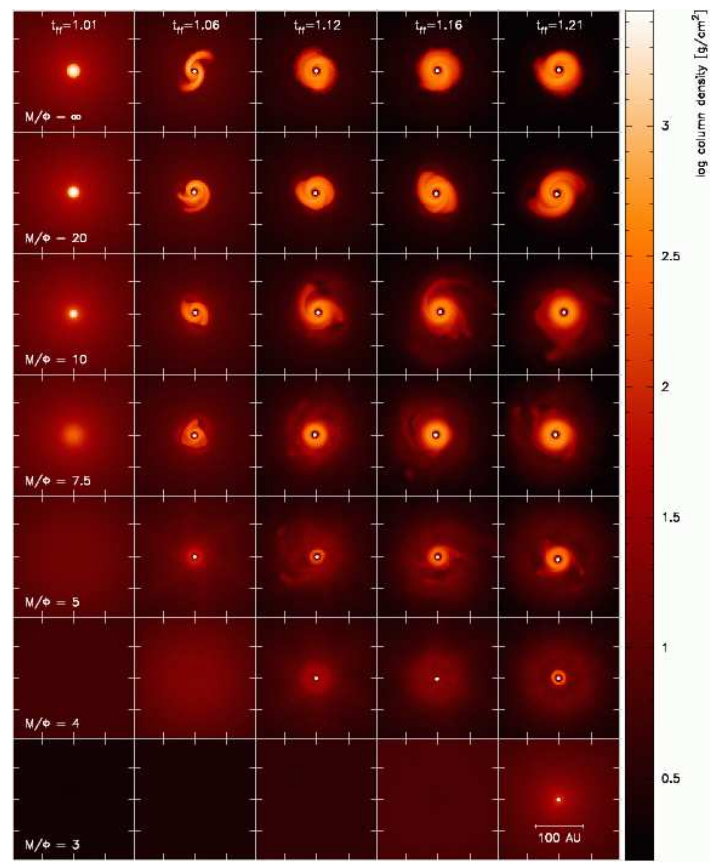
\includegraphics[height=0.6\textheight]{images/MF_disc_formation.png}
\caption{Effect of magnetic field of disc formation}
\label{MF}
\end{figure}

We see in Figure \ref{MF} above the evolution of stars over time with various magnetic field strengths (the mass-to-flux ratio $\frac{M}{\phi}$ decreases from top to bottom, corresponding to increasing magnetic field strength). From this figure we see that ``increasing the magnetic field strength tends to delay and also suppress disc formation''\cite{PriceAndBate}.



\pagebreak

\subsection{Research Task 3}
\begin{framed}
There is strong evidence for `solar-sized' black holes. What is the best evidence for these black holes and merged to emit the gravity waves detected by LIGO were 29 and 35 solar masses. Comment on how this discovery fits with what we already know about black hole masses.
\end{framed}

The best evidence for these black holes is data collected from x-ray binaries \cite{Casares} (XRB), where a giant or supergiant star acretes stellar material onto a compact binary companion; during which, the stellar material is heated and gives off x-rays. From this data, the motion and masses of the binary objects can be determined.

To date, 22 solar-sized black holes have been discovered, 19 of which are inside the Milky Way with masses ranging from $\sim 3 - \ms{20}$ \cite{Abbot}. The first of these was a binary system called Cygness X-1, discovered in the late 1960's  \cite{Casares}.

The predicted range of solar-sized black holes is from $\sim 3 - \ms{80}$ (see Fig 1. of \cite{Abbot}). The latest data from the LIGO Binary Black Hole (BBH) merger fits well with the currently predicted masses of black holes, as it shows that larher mass black holes as it shows that larger mass black holes do actually exist in the universe.

Although they are the largest ones to be verified. These are two extragalactic XRBs that have masses in the range of $21 - \ms{35}$ and $12 - \ms{24}$, however the data is considered unreliable \cite{Abbot}.

\pagebreak

\section{Conclusion}
\begin{framed}
In your conclusions please consider how the black holes seen by LIGO might have formed. Although you should have not done a full suite of calculations, you should have a few ideas about what the issues might be in forming this pair of black holes. How likely do you think they might be?
\end{framed}

The majority of the solar-sized black holes detected to date have been found in XRB systems with masses ranging from $\sim 3- \ms{20}$. However, with the LIGO detector, it is now possible to detect BBHs through the emission of gravitational waves. The data, whichs shows the merger between a $\SI{29}{M_\odot}$ and $\SI{35}{M_\odot}$ black holes is the first data to confirm that tere are larger BH masses than the ones detected so far. It seems unlikely that such large BHs could be formed by XRBs, although not completely ruled out. It is more likely that BBH systems are formed in densely populatied stellar environments such as globual clusters. Another possible method of formation is through rogue BH capture, but this is probably even rarer than large mass XRB BHs. With the accumulation of more data from LIGO these question will eventually be answered.

\pagebreak

\section{References}

\bibliographystyle{plain}
\bibliography{refs.bib}


\end{document}



























